\chapter{Digit classifier}\label{ch:digitclass}
Taking advantage of the \glspl{cnn} impressive performance in classification tasks, we have built a \textbf{real-time digit classifier} which captures images from any video stream, applies the necessary preprocessing and displays the predicted digit.

These are the major challenges that have been overcome during the development of the application:
\begin{itemize}
	\item Understanding \textbf{how the \glspl{cnn} are built} with Keras.
	\item Developing a \textbf{component} for the application.
	\item Creating a \textbf{dataset} with images that resemble the ones found in the real world.
	\item Building a \textbf{benchmark} to evaluate the performance of the \glspl{cnn}.
	\item Finding the \textbf{optimal \gls{cnn} model}: architecture and learning process.
\end{itemize}

\section{Understanding the Keras model}\label{sec:classifier}
The starting point for the digit classifier is a \textbf{Keras example} that can be accessed from its GitHub \footnote{\url{https://git.io/vH0qw}}. In that example, a \gls{cnn} is trained and tested with the \textbf{MNIST dataset} (see Section~\ref{subsec:MNIST}). That code has been used to take the first steps in this project and an adapted version of it \footnote{\url{https://git.io/vH0qK}} is going to be analyzed in the following sections.

\subsection{Preparing data}\label{subsec:adaptdata}
First of all, the input data has to be \textbf{loaded} and \textbf{adapted}. Keras library contains a module named \textbf{\textit{datasets}} from which a variety of databases can be imported, including MNIST. The MNIST database can be loaded calling the \textbf{\textit{mnist.load\_data()} method}. It returns, as \textbf{Numpy arrays}, the images and labels from both training and test datasets. The code can be seen in the following frame:
\begin{lstlisting}
    '''
    Loading and shaping data in a way that it can work as input of our model
    '''
    # MNIST data
    (x_train, y_train), (x_test, y_test) = mnist.load_data()
    
    cv2.imshow('First sample',x_train[0])
    cv2.waitKey(5000)
    cv2.destroyWindow('First sample')
    
    print ('Original input images data shape: ', x_train.shape) 
\end{lstlisting}

In Figure~\ref{fig:firstsample}, the first sample of the MNIST training dataset, as displayed by the code above, can be seen. That code also prints the shape of the dataset:
\begin{Verbatim}[frame=single]
Original input images data shape:  (60000, 28, 28)
\end{Verbatim}

\begin{figure}
	\centering
	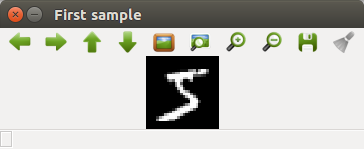
\includegraphics[width=0.7\linewidth, keepaspectratio]{figures/first_sample.png}
	\caption{First sample of the MNIST database.}
	\label{fig:firstsample}
\end{figure}

This means that the training dataset includes 60000 images, each one containing 28x28 pixels. In order to feed a Keras model (see Section~\ref{subsec:models}), the \textbf{number of channels} of the samples have to be explicitly declared as well, so the dataset must be \textbf{reshaped}. In this case, the samples are \textbf{grayscale images}, which implies that the number of channels is equal to 1. For instance, if they had been RGB images, the number of channels would have been equal to 3. As data is stored in Numpy arrays, it can be reshaped using the \textbf{\textit{.reshape()} method}. The order in which dimensions must be declared depends on the \textbf{\textit{.image\_dim\_ordering()} parameter} of the Keras \textit{backend}, as it can be seen in the following frame:
\begin{lstlisting}
    if backend.image_dim_ordering() == 'th':
    # reshapes 3D data provided (nb_samples, width, height) into 4D
    # (nb_samples, nb_features, width, height) 
	    x_train = x_train.reshape (x_train.shape[0], 1, img_rows, img_cols)
	    x_test = x_test.reshape (x_test.shape[0], 1, img_rows, img_cols)
	    input_shape = (1,img_rows,img_cols)
	    print ('Input images data reshaped: ', (x_train.shape))
	    print ('--------------------------------------------------------------')
    else:
    # reshapes 3D data provided (nb_samples, width, height) into 4D
    # (nb_samples, nb_features, width, height) 
	    x_train = x_train.reshape(x_train.shape[0], img_rows, img_cols, 1)
	    x_test = x_test.reshape(x_test.shape[0], img_rows, img_cols, 1)
	    input_shape = (img_rows, img_cols, 1)
	    print ('Input images data reshaped: ', (x_train.shape))
	    print ('--------------------------------------------------------------')
\end{lstlisting}
 
In this case, the input data gets reshaped as follows:
\begin{Verbatim}[frame=single]
Input images data reshaped:  (60000, 28, 28, 1)
\end{Verbatim}

The last step to get the input images ready is to \textbf{convert data type} from \textit{uint8} to \textit{float32} and \textbf{normalize pixel values} to [0,1] range:
\begin{lstlisting}
    # converts the input data to 32bit floats and normalize it to [0,1]
    print('Input images type: ',x_train.dtype)
    x_train = x_train.astype('float32')
    x_test = x_test.astype('float32')
    print('New input images type: ',x_train.dtype)
    print ('-----------------------------------------------------------------')
    x_train /= 255
    x_test /= 255
\end{lstlisting}

Finally, the \textbf{labels} have to be reshaped from an array in which each element is an integer in the range [0, 9] to an array in which each element is \textbf{an array of probabilities}. E.g.,  if the element of the original array is 2, in the reshaped array it will be [0, 0, 1, 0, 0, 0, 0, 0, 0, 0]. This conversion is achieved using the Keras built-in method \textbf{\textit{np\_utils.to\_categorical()}}:
\begin{lstlisting}
    print ('First 10 class labels: ', (y_train[:10]))
    print ('Original class label data shape: ', (y_train.shape))
    # converts class vector (integers from 0 to nb_classes) to class matrix
    # (nb_samples, nb_classes)
    y_train = np_utils.to_categorical(y_train, nb_classes)
    y_test = np_utils.to_categorical(y_test, nb_classes)
    print ('Class label data reshaped: ', (y_train.shape))
    print ('-----------------------------------------------------------------')
\end{lstlisting}

This code prints:
\begin{Verbatim}[frame=single]
First 10 class labels:  [5 0 4 1 9 2 1 3 1 4]
Original class label data shape:  (60000,)
Class label data reshaped:  (60000, 10)
\end{Verbatim}

\subsection{Model architecture}
Once the data is ready, it's time to define the architecture of the \gls{cnn}. In this example, a \textbf{sequential model} (see Section~\ref{subsec:models}) is enough for solving the classification task and it is declared as follows:
\begin{lstlisting}
    # defines the model architecture, in this case, sequential
    model = Sequential()
\end{lstlisting}

The next step is to add the corresponding layers. The core layers of a \gls{cnn}, as treated by Keras, have been already defined in Section~\ref{subsec:layers}. The following code performs the addition of the layers to the model:
\begin{lstlisting}
    '''
    Adding layers to our model
    '''
    # convolutional layer
    model.add(Convolution2D(nb_filters, kernel_size[0], kernel_size[1],
			    border_mode='valid', input_shape=input_shape, 
			    activation='relu'))
    # convolutional layer
    model.add(Convolution2D(nb_filters, kernel_size[0], kernel_size[1],
			    activation='relu'))
    # pooling layer
    model.add(MaxPooling2D(pool_size=pool_size))
    # dropout layer
    model.add(Dropout(0.25))
    
    # flattening the weights (making them 1D) to enter fully connected layer
    model.add(Flatten())
    # fully connected layer
    model.add(Dense(128, activation='relu'))
    # dropout layer to prevent overfitting
    model.add(Dropout(0.5))
    # output layer
    model.add(Dense(nb_classes, activation='softmax'))
\end{lstlisting}

As defined by the code above, the model is formed by the following layers:
\begin{itemize}
	\item A \textbf{2D convolutional layer} with 32 filters whose size is 3x3x1.
	\begin{itemize}
		\item Since this is the first layer of the model, the \textbf{\textit{input\_shape}} argument must be provided. In this case, the input shape is 28x28x1. 
		\item As \textit{valid} mode is set, \textbf{no padding} is applied and the output dimension will be reduced. 
		\item \textbf{\gls{relu} activation function} (see Equation~\ref{eq:relu}) introduces non-linearity into the network. If the activation functions were linear, the whole stack of layers could be reduced to a single layer, losing much of the ability to learn different levels of features.
		\item This layer outputs 32 activation maps with size 26x26.
	\end{itemize}
		
	\item Another \textbf{convolutional layer} with the \textbf{same arguments}: 32 filters, no padding and \gls{relu} as activation function.
	\begin{itemize}
		\item Increasing the number of convolutional layers allows the \gls{cnn} to learn \textbf{more complex features}. 
		\item As the \textbf{depth} of its input is 32 (one channel per activation map), the size of the filters will be 3x3x32. 
		\item This layer outputs 32 activation maps with size 24x24.
	\end{itemize}
	
	\item A \textbf{2D MaxPooling layer} with a \textbf{\textit{pool\_size}} of 2x2.
	\begin{itemize}
		\item This layer outputs the 32 activation maps generated by the previous layer, but \textbf{\textit{downsampled}} by a factor of 2, resulting in maps with size 12x12.
	\end{itemize}
	
	\item A \textbf{dropout layer} to prevent \textbf{overfitting}. 
	\begin{itemize}
		\item The fraction of random units that are going to be \textbf{\textit{swicthed-off}} is 0.25.
		\item This layer preserves the size and the shape of its input.
	\end{itemize} 
	
	\item A \textbf{flatten layer} that turns the matrices of weights that it receives at its input into a vector that can be fed to the fully-connected layer.
	\item A fully-connected or \textbf{dense layer}.
	\begin{itemize}
		\item This layer contains 128 neurons that will output an array of 128 values.
		\item Once more, the \textbf{\gls{relu} activation function} is applied.
	\end{itemize} 
	
	\item A \textbf{dropout layer} with a 0.5 fraction.
	
	\item Finally, the \textbf{output layer} is another \textbf{dense layer} which contains as many neurons as classes, in this example, 10. 
	\begin{itemize}
		\item In order to output a \textbf{probability distribution} of the predicted classes, the activation function will be \textbf{softmax} (Equation~\ref{eq:SoftMax}).
	\end{itemize}
\end{itemize}

The resulting architecture and the shape of the data as it goes through every layer can be seen in Figure~\ref{fig:model}.

\begin{figure}
	\centering
	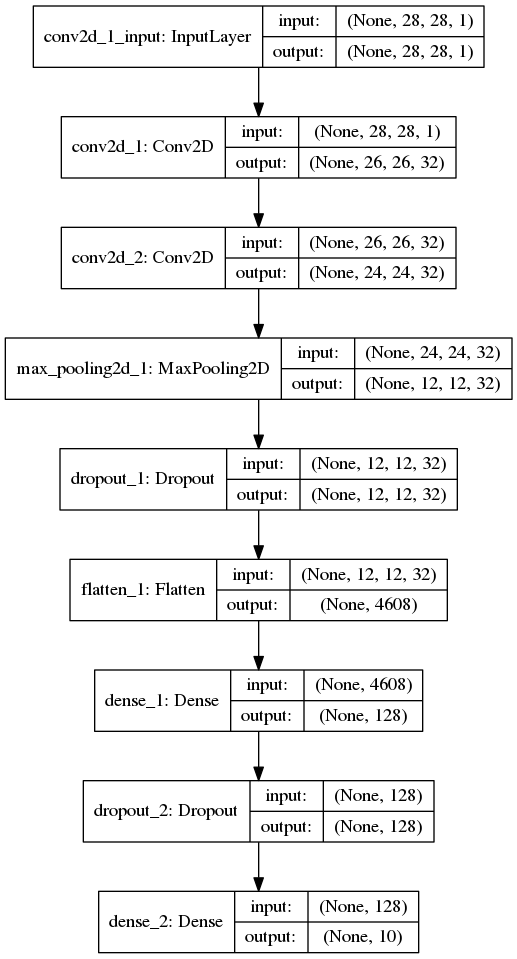
\includegraphics[width=0.75\linewidth, keepaspectratio]{figures/model.png}
	\caption{Diagram of a Keras sequential model.}
	\label{fig:model}
\end{figure}

\subsection{Compiling the model}
After declaring the model and defining its architecture, the \textbf{learning process} must be compiled. The arguments required to set this process are defined in Section~\ref{subsec:models}. The code can be seen in the next frame:
\begin{lstlisting}
    '''
    Compiling the model
    '''
    model.compile(loss='categorical_crossentropy', optimizer='adadelta', 
				    metrics=['accuracy'])
\end{lstlisting}

For this example, the loss function that is computed after every batch is the \textbf{categorical cross-entropy} (see Equation~\ref{eq:categorical_crossentropy}) and the optimizer that updates the weights of the \gls{cnn} in order to minimize that loss function is \textbf{ADADELTA} (see Algorithm~\ref{adadelta}). Additionally, the \textbf{accuracy} is also computed to monitor \textbf{the \gls{cnn} performance} during training.

\subsection{Training the model}
The \gls{cnn} is trained thanks to the \textbf{\textit{.fit()} method}, which has been already described in Section~\ref{subsec:models}. The code below shows how it is called:
\begin{lstlisting}
    '''
    Training the model
    '''
    model.fit(x_train, y_train, batch_size=batch_size, nb_epoch=nb_epoch,
			    verbose=1, validation_data=(x_test, y_test))
\end{lstlisting}

The model that has been built is trained for 12 \textbf{epochs} and the \textbf{batch size}, i.e., the number of samples that pass through the \gls{cnn} before updating the weights, is 128. The test dataset is used here as \textbf{validation data} for which the log loss and the accuracy will be computed after every epoch just for \textbf{monitoring purposes}. During training time, Keras prints the results after every batch and epoch as follows:
\begin{Verbatim}[frame=single]
Train on 60000 samples, validate on 10000 samples
Epoch 1/12
128/60000 [....................] - ETA: 350s - loss: 2.3223 - acc: 0.1016
256/60000 [....................] - ETA: 312s - loss: 2.3073 - acc: 0.1094
384/60000 [....................] - ETA: 287s - loss: 2.2927 - acc: 0.1458
...
59648/60000 [==================>.] - ETA: 2s - loss: 0.0455 - acc: 0.9871
59776/60000 [==================>.] - ETA: 1s - loss: 0.0455 - acc: 0.9871
59904/60000 [==================>.] - ETA: 0s - loss: 0.0455 - acc: 0.9871
60000/60000 [====================] - 407s - loss: 0.0455 - acc: 0.9871 - 
val_loss: 0.0306 - val_acc: 0.9891
\end{Verbatim}

\subsection{Testing the model}
Once the model is trained, we can store its weights, architecture and learning configuration in a \textbf{HDF5 file} (see Section~\ref{sec:hdf}). Besides that, in order to see the performance of the \gls{cnn}, the \textbf{\textit{.evaluate()} method} takes the test dataset and computes the log loss and the accuracy. Both storing and evaluation processes can be seen in the following code:
\begin{lstlisting}
    '''
    Saving the model architecture and weights
    '''
    model.save('MNIST_net.h5')
    
    '''
    Testing the model
    '''
    score = model.evaluate(x_test, y_test, verbose=0)
    print('Test score:', score[0])
    print('Test accuracy:', score[1])
\end{lstlisting}
These are the results obtained with this example (\textit{Test score} refers to loss):
\begin{Verbatim}[frame=single]
Test score: 0.0306129640532
Test accuracy: 0.9891
\end{Verbatim}

\section{Component}\label{sec:component}
Once the neural network has been trained and the resultant model is saved, the next milestone is to integrate it into a component that must be able to \textbf{get images} from a video stream and \textbf{display the predictions} obtained from them. That component is \textbf{\textit{digitclassifier.py}} \footnote{\url{https://git.io/vH0qi}} and it is based on Nuria Oyaga code \footnote{\url{https://git.io/vH0qD}}. \textit{digitclassifier.py} depends on two classes: \textbf{\textit{Camera}} and \textbf{\textit{GUI}}. Figure~\ref{fig:digitclass} shows the program running.

\begin{figure}
	\centering
	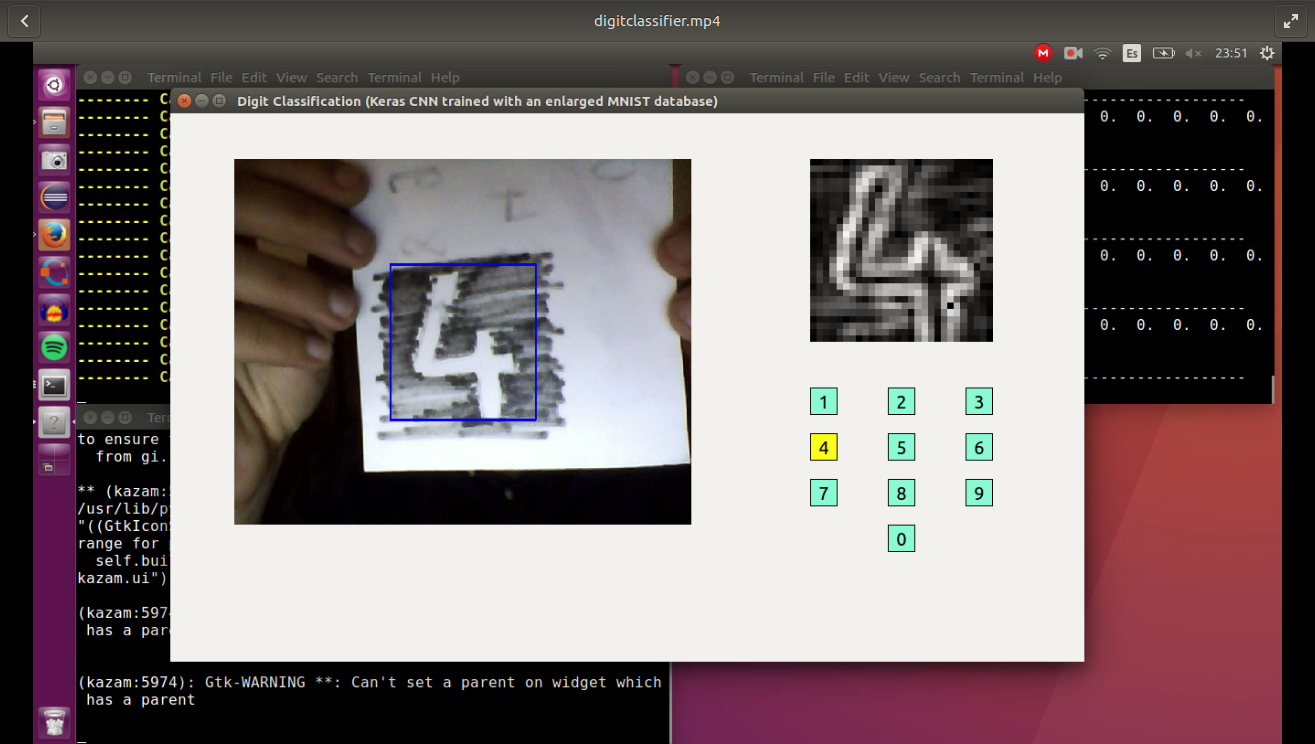
\includegraphics[width=1\linewidth, keepaspectratio]{figures/digitclass.png}
	\caption{Example of \textit{digitclassifier.py} execution.}
	\label{fig:digitclass}
\end{figure}

\subsection{\textit{Camera} class}
\textbf{\textit{Camera} class} \footnote{\url{https://git.io/vH0qS}} is responsible for getting the images, transforming them into a suitable input for the Keras model and returning the classification results.

\begin{itemize}
	\item \textbf{Acquisition}. The images are served by the JdeRobot component \textbf{\textit{cameraserver}} (see Section~\ref{sec:jderobot}). Depending on how its \textbf{configuration file} (\textit{cameraserver.cfg}) has been set, the images can come from different kinds of video streams. During the development of this application, the digit classifier component has been tested with \textbf{webcams}, \textbf{video files} and \textbf{smartphone cameras}. Connection with webcams and video files is straightforward: the URI property in the configuration file must be changed to the number of device or the path of the video, as it can be seen in the code below.
	\begin{lstlisting}[frame=single]
	#0 corresponds to /dev/video0, 1 to /dev/video1, and so on...
	#CameraSrv.Camera.0.Uri=1                                # webcam
	CameraSrv.Camera.0.Uri=/home/dpascualhe/video.mp4        # video file
	\end{lstlisting}
	
	In order to establish a connection with smartphone cameras, the \textbf{DroidCam application} (see Section~\ref{sec:droidcam}) for Android has been used. As this application turns the video stream provided by the smartphone into a \textbf{v4l2 \footnote{\url{https://www.linuxtv.org/wiki/index.php/Main_Page}} device driver}, the video stream will be listed as another webcam and the number of device must be set in the \textit{cameraserver} configuration file.
	
	Besides that, the \textbf{address} at which the video is being served by the \textit{cameraserver} component is provided to the \textit{Camera} class thanks to another configuration file: \textbf{\textit{digitclassifier.cfg}} \footnote{\url{https://git.io/vH0zi}}.
	
	\item \textbf{Preprocessing}. As the images can be captured with \textbf{different devices}, the \textit{digitclassifier.py} component must apply some preprocessing that mitigates the differences between video streams and that makes the images \textbf{suitable for the Keras model}. The following \textbf{transformations} are applied before classification:
	\begin{enumerate}
		\item Images are \textbf{cropped} into 80x80 pixels images. The \textbf{\gls{roi}} from which cropped images are extracted is \textbf{draw over the original image}, making it easier to aim at digits with the camera.
		\item Color doesn't provide any useful information about digits and MNIST database is formed by \textbf{grayscale images}. For this reason, the images captured with the component are converted into grayscale images as well. 
		\item A \textbf{Gaussian filtering} is applied in order to \textbf{reduce image noise}. When using this operator, the \textbf{kernel size} and the \textbf{standard deviation} $\sigma$ in $x$ and $y$ should be specified~\cite{itseez2014theopencv}. In this case, the kernel size will be 5x5 and the standard deviation is automatically calculated depending on that size. The 2D Gaussian filter, as defined in~\cite{sonka1999image}, is given by:
		\begin{equation}
		G(x,y)=\exp(-\frac{x^2+y^2}{2\sigma^2})
		\end{equation}
		\item After reducing noise, the image is \textbf{resized} to fit the Keras \textbf{model input}. The new size is 28x28 pixels, like MNIST samples.
		\item Last step is obtaining the \textbf{gradient of the images}. Working with this kind of images instead of the original ones allows the application to deal with \textbf{different light and color conditions}. The chosen algorithm for this task is \textbf{Sobel filter} (Equation~\ref{eq:sobel}). This will be deeply discussed in Section~\ref{subsec:edge}.
	\end{enumerate}
	
	The following code applies the transformations mentioned above:
	\begin{lstlisting}[frame=single]
		def trasformImage(self, im):
			''' Transforms the image into a 28x28 pixel grayscale image and
			applies a sobel filter (both x and y directions).
			''' 
			im_crop = im [140:340, 220:420]
			im_gray = cv2.cvtColor(im_crop, cv2.COLOR_BGR2GRAY)
			im_blur = cv2.GaussianBlur(im_gray, (5, 5), 0) # Noise reduction.
			
			im_res = cv2.resize(im_blur, (28, 28))
			 
			# Edge extraction.
			im_sobel_x = cv2.Sobel(im_res, cv2.CV_32F, 1, 0, ksize=5)
			im_sobel_y = cv2.Sobel(im_res, cv2.CV_32F, 0, 1, ksize=5)
			im_edges = cv2.add(abs(im_sobel_x), abs(im_sobel_y))
			im_edges = cv2.normalize(im_edges, None, 0, 255, cv2.NORM_MINMAX)
			im_edges = np.uint8(im_edges)
			 
			return im_edges
	\end{lstlisting}
	
	\item \textbf{Classification}. Before entering the \gls{cnn}, the images are \textbf{reshaped} as mentioned in Section~\ref{subsec:adaptdata}. \textit{Camera} class calls Keras \textbf{\textit{.predict()} method} (see Section~\ref{subsec:models}) to get the predicted digit. Finally, the case in which prediction doesn't return a clear answer is handled. This process can be seen in the following code:
	\begin{lstlisting}
	    def classification(self, im):
	    ''' Adapts image shape depending on Keras backend (TensorFlow
	    or Theano) and returns a prediction.
	    '''
	    if backend.image_dim_ordering() == 'th':
		    im = im.reshape(1, 1, im.shape[0], im.shape[1])            
	    else:      
		    im = im.reshape(1, im.shape[0], im.shape[1], 1)            
	    
	    dgt = np.where(self.model.predict(im) == 1)
	    print("Keras \gls{cnn} prediction: ", self.model.predict(im))
	    print("Prediction index: ", dgt)
	    print("-----------------------------------------------------------")
	    if dgt[1].size == 1:
		    self.digito = dgt
	    else:
		    self.digito = (([0]), (["none"]))
	    
	    return self.digito[1][0]
	\end{lstlisting}
\end{itemize}

\subsection{\textit{GUI} class}
\textbf{\textit{GUI} class} \footnote{\url{https://git.io/vH0YK}} displays the \textbf{original image}, the \textbf{processed image} and the result of the \textbf{classification}, as it can be seen in Figure~\ref{fig:digitclass}. It has been built employing the \textbf{pyQt package} \footnote{\url{https://pypi.python.org/pypi/PyQt4}} \footnote{\url{https://pypi.python.org/pypi/PyQt4}}. It is based in Nuria Oyaga code \footnote{\url{https://git.io/vH0mx}}, but it has been updated from Qt4  to Qt5  thanks to the information provided by its documentation~\cite{pyqt5}.

\subsection{Threads} 
In order to capture images and update the GUI \textbf{concurrently}, the \textbf{\textit{threading} module}~\cite{threading}, provided by Python, has been employed. From this module, a subclass of the \textbf{\textit{Thread} object} is created. In this new subclass, \textit{\_\_init\_\_()} and \textit{.run()} methods are overriden. The \textit{.run()} method is responsible for calling a process which must \textbf{update the thread}. For example, the \textit{.update()} method of the \textit{Camera} class, which reads a new image from the video stream each time it is invoked, is called within the \textit{.run()} method of the \textbf{\textit{ThreadCamera} class}. Besides that, in the \textit{.run()} method, the \textbf{cycle time} is adjusted. The next frame shows how the \textit{ThreadCamera} class is coded:
\begin{lstlisting}
import time
import threading
from datetime import datetime

t_cycle = 150  # ms

class ThreadCamera(threading.Thread):

def __init__(self, cam):
	''' Threading class for Camera. '''
	self.cam = cam
	threading.Thread.__init__(self)

def run(self):
	''' Updates the thread. '''
	while(True):
		start_time = datetime.now()
		self.cam.update()
		end_time = datetime.now()
		
		dt = end_time - start_time
		dtms = ((dt.days * 24 * 60 * 60 + dt.seconds) * 1000
					+ dt.microseconds / 1000.0)
		
		if(dtms < t_cycle):
			time.sleep((t_cycle - dtms) / 1000.0);
\end{lstlisting}
This code, as well as the one corresponding to the \textbf{\textit{ThreadGUI} class}, can be accessed in GitHub \footnote{\url{https://git.io/vH0lY}} \footnote{\url{https://git.io/vH0lW}}.

\subsection{Main program}
All of these elements are joined together in \textbf{\textit{digitclassifier.py}}. \textit{Camera} and \textit{GUI} classes and their threads are initialized and the \textbf{\textit{.start()}} methods of the \textit{Thread} objects are invoked, as it can be seen in the code below:
\begin{lstlisting}
if __name__ == '__main__':

	cam = Camera()
	app = QtWidgets.QApplication(sys.argv)
	window = GUI()
	window.setCamera(cam)
	window.show()
	
	# Threading camera
	t_cam = ThreadCamera(cam)
	t_cam.start()
	
	# Threading GUI
	t_gui = ThreadGUI(window)
	t_gui.start()
	
	sys.exit(app.exec_())
\end{lstlisting}

In order to execute the program:
\begin{enumerate}
	\item \textit{cameraserver} must be launched with its configuration file as an argument in a terminal:
\begin{Verbatim}[frame=single]
dpascualhe@hp-g6:~$ cameraserver cameraserver.cfg
\end{Verbatim}
	
	\item In another terminal, \textit{digitclassifier.py} must be launched with its configuration file as well:
\begin{Verbatim}[frame=single]
dpascualhe@hp-g6:~$ python digitclassifier.py digitclassifier.cfg
\end{Verbatim}
\end{enumerate}

An example of usage of the digit classifier component can be seen in Figure~\ref{fig:digitclass}.

\section{Datasets}\label{sec:datasets}
The digit classifier component is possible thanks to the data provided by the \textbf{MNIST database} of handwritten digits~\cite{lecun-mnisthandwrittendigit-2010}. In the following sections, the pros and cons of using this database and some alternatives will be discussed.

\subsection{Original dataset}\label{subsec:MNIST}
\textbf{MNIST (Modified National Institute of Standards and Technology database)}~\cite{lecun-mnisthandwrittendigit-2010} is a database of \textbf{handwritten digits} formed by a training set, which contains 60000 samples, and a test set, containing 10000 samples. It's a \textit{remixed} and reduced version of the original \textbf{NIST datasets} \footnote{\url{https://www.nist.gov/srd/nist-special-database-19}}. MNIST is a well-known \textbf{benchmark} for all kinds of machine learning algorithms.

As may be seen in Figure~\ref{fig:mnist}, each sample of the MNIST database is a 28x28 pixels \textbf{grayscale image} that contains a \textbf{size-normalized} and \textbf{centered} digit. While it may be useful for testing machine learning algorithms, it's not enough to train a model that aims to solve a \textbf{real-world task}, because the images are almost noiseless and share similar orientation, position, size and intensity levels.
\begin{figure}
	\centering
	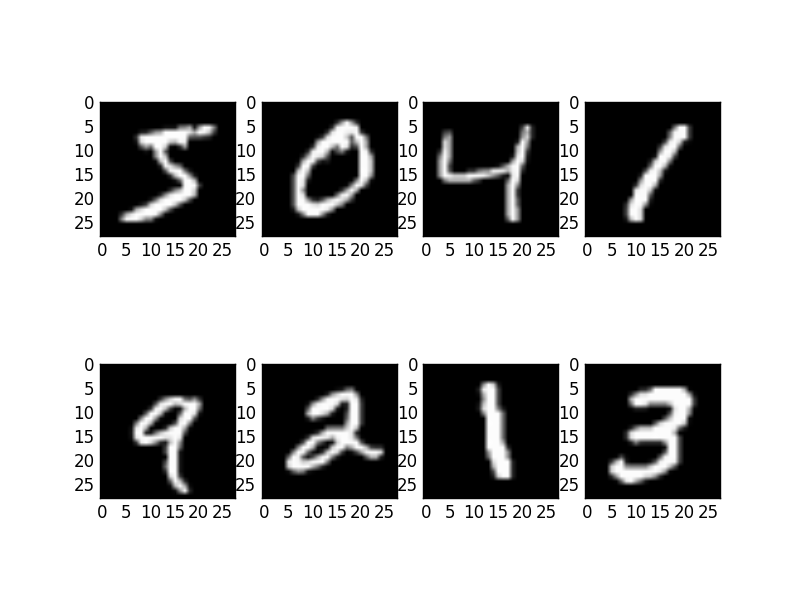
\includegraphics[width=12cm, keepaspectratio]{figures/mnist.png}
	\caption{Samples extracted from the MNIST database.}
	\label{fig:mnist}
\end{figure}

\subsection{Gradient images}\label{subsec:edge}
The first issue with MNIST database that must be addressed is that the grayscale images that it contains share \textbf{similar intensity levels}: a white digit over a black background. In real world, the digits can be found written in several colors over different backgrounds and the datasets must resemble every possible combination. In order to achieve that generalization, the \textbf{gradient of the images} has been calculated. The resultant samples are less dependent from the light and color conditions than the original ones, forcing the neural network to focus in the shape of the digits to classify them.

According to the study carried out by Nuria Oyaga \footnote{\url{http://jderobot.org/Noyaga-tfg\#Testing\_Neural\_Network}}, the operator that leads to better results is the \textbf{Sobel filter}. This operator approximates the \textbf{gradient} of an image function~\cite{sonka1999image}, convolving the image with the following \textbf{kernels} to detect horizontal and vertical edges, respectively:  
\begin{equation}\label{eq:sobel}
h_x = 
\begin{bmatrix}
1 & 2 & 1\\
0 & 0 & 0\\
-1 & -2 & -1
\end{bmatrix}
,\quad
h_y = 
\begin{bmatrix}
-1 & 0 & 1\\
-2 & 0 & 2\\
-1 & 0 & 1
\end{bmatrix}
\end{equation}
The absolute values of the resultant images, $x$ and $y$, are then added, obtaining the gradient image.

\subsection{Data augmentation}
The second problem that has been detected with MNIST is that the images are \textbf{noiseless} and the digits are always centered with a scale and a rotation angle that are almost \textbf{invariant}. However, the digit classifier has to deal with noisy images that can be randomly scaled, translated and/or rotated. In order to get a database with images that look like the ones that our application is going to work with, the MNIST database must be augmented.

Two alternatives have been considered to solve this problem: \textbf{real-time data augmentation} provided by Keras and \textbf{generating our own database}.

\subsubsection{Real-time data augmentation with Keras}
Thanks to the \textbf{\textit{.ImageDataGenerator()} method} provided by Keras (see Section~\ref{subsec:utils}), the MNIST dataset can be augmented in \textbf{real-time} during training. In order to cover most of the real cases, random \textbf{rotation}, \textbf{translation} and \textbf{zooming} were applied to generate new samples. In addition to that, a \textbf{Sobel filtering} was also applied through a \textbf{user-defined function}. The samples generated by the following code \footnote{\url{https://git.io/vH0qz}} can be seen in Figure~\ref{fig:aug_keras}.
\begin{lstlisting}
	if mode == "full":
		datagen = imkeras.ImageDataGenerator(
			zoom_range=0.2, rotation_range=20, width_shift_range=0.2, 
			height_shift_range=0.2, fill_mode='constant', cval=0,
			preprocessing_function=self.sobelEdges)
	elif mode == "edges":
		datagen = imkeras.ImageDataGenerator(
			preprocessing_function=self.sobelEdges)

generator = datagen.flow(x, y, batch\_size=batch\_size)
\end{lstlisting}

\begin{figure}
	\centering
	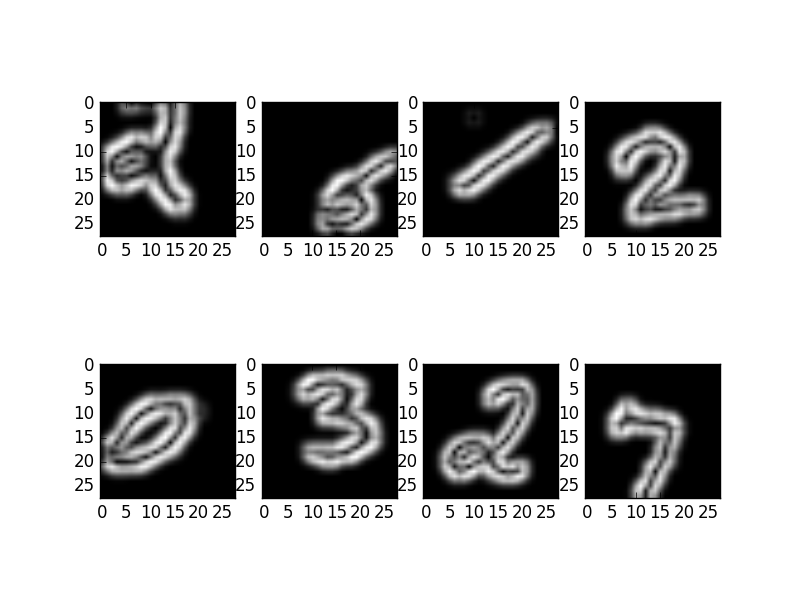
\includegraphics[width=12cm, keepaspectratio]{figures/aug_keras.png}
	\caption{Samples generated with Keras from MNIST database.}
	\label{fig:aug_keras}
\end{figure}

Besides these transformations, it's also necessary to simulate the \textbf{noise} that may be present in real images. Keras generator doesn't support the addition of noise. For this purpose, Keras includes noise layers such as the \textbf{GaussianNoise layer}, which adds Gaussian noise with a standard deviation distribution defined by the user. It's important to note that Keras treat noise layers as regularization methods that are only active during training time to avoid overfitting. In order to add noise to the generated samples, a GaussianNoise layer was established as the \textbf{input layer} of the model.

\subsubsection{Handmade augmented datasets}
The alternative to real-time data augmentation with Keras is building \textbf{our own datasets} applying the previously mentioned transformations to the images. My mate Nuria Oyaga has build 5 new databases with two sets each one: training and validation \footnote{\url{http://jderobot.org/Noyaga-tfg\#Comparing_Neural_Network}}. These are the new databases: 
\begin{itemize}
	\item \textbf{Sobel}: MNIST database after applying the Sobel filter to every image. 48000 samples for traning and 12000 samples for validation. 
	\item \textbf{0-1}: Same size than Sobel database. One transformed image per every Sobel database image. Sobel database images are replaced by the the transformed ones. 48000 samples for traning and 12000 samples for validation. 
	\item \textbf{1-1}: Double size than Sobel database. One transformed image per every Sobel database image. Both Sobel database images and the transformed images are included in the 1-1 database. 96000 samples for training and 24000 samples for validation. 
	\item \textbf{0-6}: Six times the size of Sobel database. Six transformed images per every Sobel database image. Sobel database images are replaced by the transformed ones. 288000 samples for training and 72000 samples for validation. 
	\item \textbf{1-6}: Seven times the size of Sobel database. Six transformed images per every Sobel database image. Both Sobel database images and the transformed images are included in the 1-6 database. 336000 samples for training and 84000 samples for validation. 
\end{itemize}

Besides that, the test dataset of the MNIST database (10000 samples) has been converted into a \textbf{1-6 test dataset} (70000 samples).

In Figure~\ref{fig:aug_nuria}, the first samples of every handmade dataset can be seen.

\begin{figure}
	\centering
	\begin{subfigure}{0.5\textwidth}
		\centering
		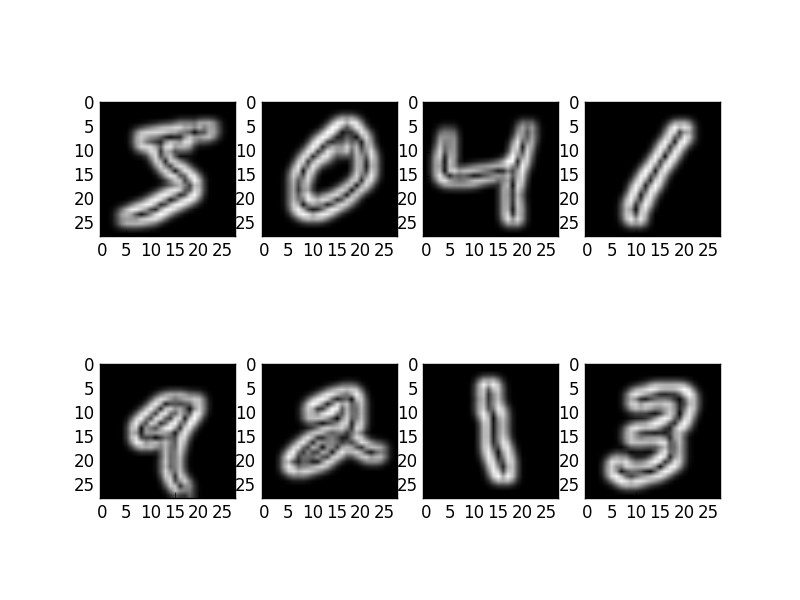
\includegraphics[width=1\linewidth]{figures/Sobel.png}
		\caption{Sobel dataset.}\label{fig:sobel}
	\end{subfigure}%
	\begin{subfigure}{0.5\textwidth}
		\centering
		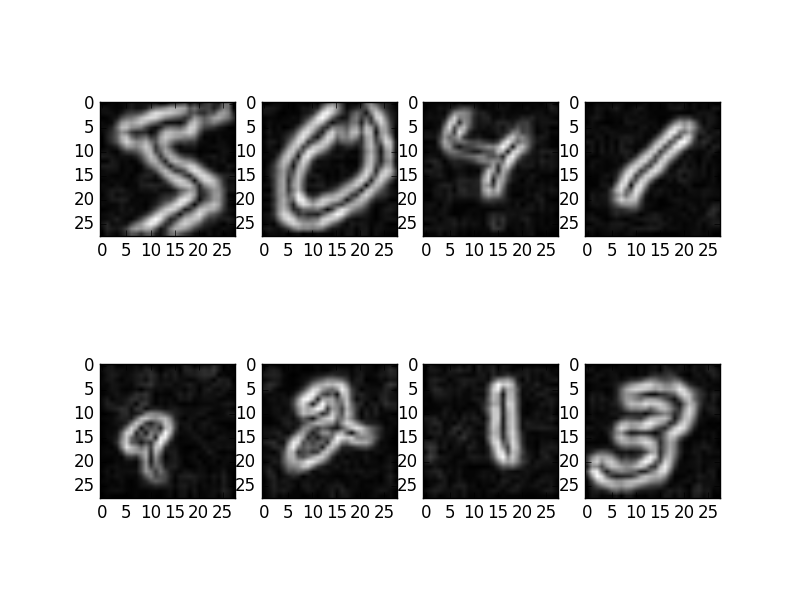
\includegraphics[width=1\linewidth]{figures/0-1.png}
		\caption{0-1 dataset.}\label{fig:0-1}
	\end{subfigure}
	\begin{subfigure}{0.5\textwidth}
		\centering
		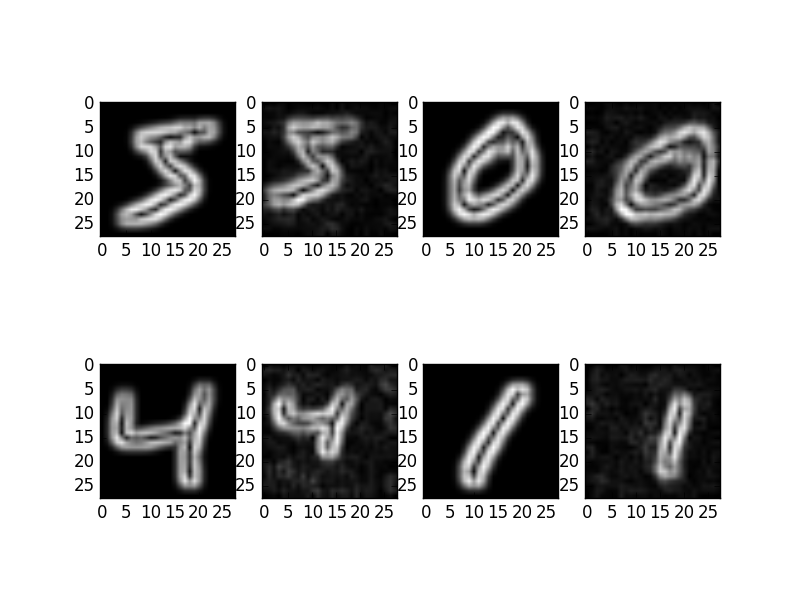
\includegraphics[width=1\linewidth]{figures/1-1.png}
		\caption{1-1 dataset.}\label{fig:1-1}
	\end{subfigure}%
	\begin{subfigure}{0.5\textwidth}
		\centering
		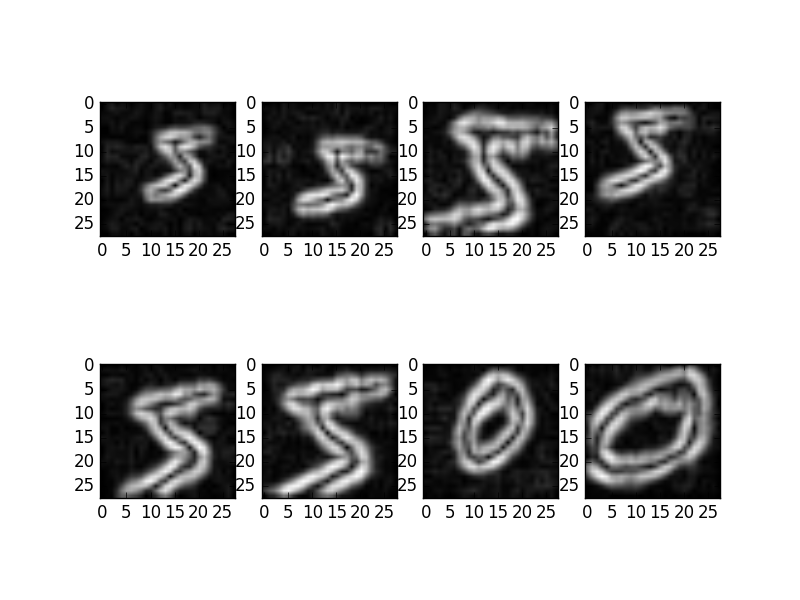
\includegraphics[width=1\linewidth]{figures/0-6.png}
		\caption{0-6 dataset.}\label{fig:0-6}
	\end{subfigure}
	\begin{subfigure}{0.5\textwidth}
		\centering
		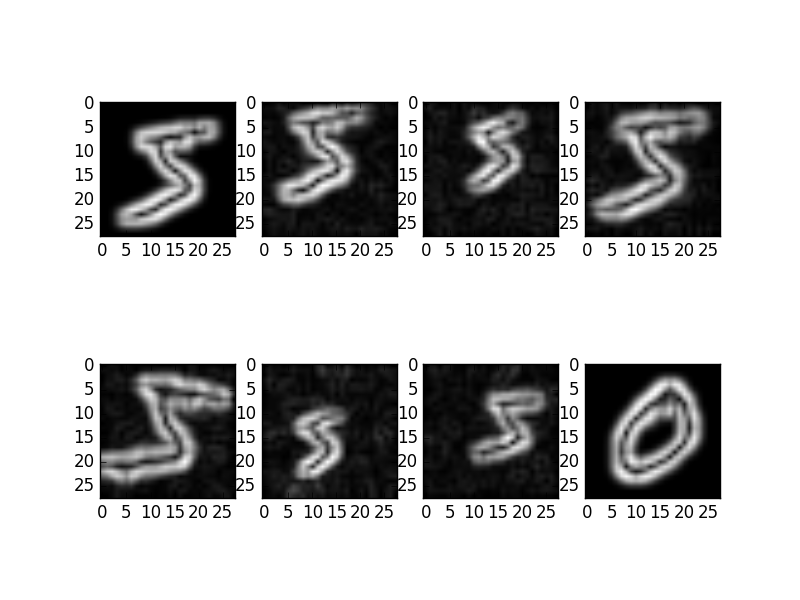
\includegraphics[width=1\linewidth]{figures/1-6.png}
		\caption{1-6 dataset.}\label{fig:1-6}
	\end{subfigure}
	\caption[First samples of handmade datasets.]{}
	\label{fig:aug_nuria}
\end{figure}

\subsubsection{From LMDB to HDF5} \label{subsubsec:lmdb2hdf5}
These databases were initially built to feed a \textbf{Caffe}~\cite{jia2014caffe} neural network. That's why they were saved as \textbf{LMDB files} \footnote{\url{http://www.lmdb.tech/doc/}}. In order to make it easier to feed the Keras model, the LMDB databases have been converted into \textbf{HDF5 files} (see Section~\ref{sec:hdf}). For this conversion, the script \textbf{\textit{datasetconversion.py}} \footnote{\url{https://git.io/vHWTe}} has been written.

\begin{itemize}
	\item \textbf{Reading the LMDB database}. The LMDB library for Python \footnote{\url{https://lmdb.readthedocs.io/en/release/\#}} was employed to open the database, initialize a cursor and iterate over each key-value pair in the database. In addition, \textbf{Google's Protocol Buffers} \footnote{\url{https://developers.google.com/protocol-buffers/}}, a.k.a. Protobuf, was used to parse the data that was extracted from the database. "With protocol buffers, you write a \textbf{\textit{.proto} description} of the data structure you wish to store. From that, the \textbf{protocol buffer compiler} creates a class that implements automatic encoding and parsing of the protocol buffer data with an efficient binary format"~\cite{protobuf}. Here can be seen the \textit{.proto} file that defines the data structure used by Caffe to store the MNIST database, as obtained from~\cite{lmdb_tutorial}: 
	\begin{lstlisting}
	package datum;
	message Datum {
		optional int32 channels = 1;
		optional int32 height = 2;
		optional int32 width = 3;
		// the actual image data, in bytes
		optional bytes data = 4;
	 	optional int32 label = 5;
	 	// Optionally, the datum could also hold float data.
	 	repeated float float_data = 6;
	 	// If true data contains an encoded image that need to be decoded
	 	optional bool encoded = 7 [default = false];
	}
	\end{lstlisting}
	 
	Thanks to the \textit{.proto} file, the compiler generates a Python module that contains the \textbf{Datum class}. Datum class provides the \textbf{\textit{.ParseFromString()} method}, which is employed to parse the image data. Here is the resulting code:
	\begin{lstlisting}
	# We initialize the cursor that we're going to use to access every
	# element in the dataset.
	lmdb_env = lmdb.open(sys.argv[1])
	lmdb_txn = lmdb_env.begin()
	lmdb_cursor = lmdb_txn.cursor()
	
	x = []
	y = []
	nb_samples = 0
	
	# Datum class deals with Google's protobuf data.
	datum = datum.Datum()
	 
	if __name__ == '__main__':
	# We extract the samples and its class one by one.
	for key, value in lmdb_cursor:
		datum.ParseFromString(value)
		label = np.array(datum.label)
		data = np.array(bytearray(datum.data))
		im = data.reshape(datum.width, datum.height,
							datum.channels).astype("uint8")
	 
		x.append(im)
		y.append(label)
		nb_samples += 1
		 
		print("Extracted samples: " + str(nb_samples) + "\n")
	 
	x = np.asarray(x)
	y = np.asarray(y)
	\end{lstlisting}

	\item \textbf{Writing the HDF5 files}. After extracting the data, it was stored in a HDF5 file. Thanks to the \textbf{h5py library} \footnote{\url{http://www.h5py.org/}} for Python, a HDF5 file with two \textit{datasets} (label and data) was created. The code can be seen in the following frame:	 
	 \begin{lstlisting}
	 f = h5py.File("../../Datasets/" + sys.argv[2] + ".h5", "w")
	 
	 # We store images.
	 x_dset = f.create_dataset("data", (nb_samples, datum.width,
									 datum.height, datum.channels), dtype="f")
	 x_dset[:] = x
	 
	 # We store labels.
	 y_dset = f.create_dataset("labels", (nb_samples,), dtype="i")
	 y_dset[:] = y
	 f.close()
	 \end{lstlisting}
\end{itemize} 

\subsubsection{Conclusions}
After coding and testing both implementations for augmenting the database, it has been decided to go for the \textbf{handmade datasets}. While real-time data augmentation is really useful to avoid storing all the data that is needed for training, it makes it harder to take a look into what is being fed to the network and reproduce results. Also, in this particular case, we are interested in \textbf{compare the performance} of neural networks built with different libraries, so they must be trained with the same datasets.

\section{Benchmark}\label{sec:bencharmk}
A \textbf{benchmark} is necessary to evaluate the results obtained when training the \glspl{cnn} with different datasets. These are the conditions that it must fulfill:
\begin{itemize}
	\item \textbf{Input}. It must be possible to use the \textbf{same datasets} with different libraries, like Keras and Caffe. For this purpose, a script that converts LMDB databases into HDF5 files has been coded. This script has been analyzed in the previous section.
	\item \textbf{Output}. \glspl{cnn} built with different libraries must be evaluated using the \textbf{same measurements} about their performance, and these measurements have to be \textbf{displayed in a uniform manner}, always employing the same visualizations. These issues are solved with \textbf{\textit{CustomEvaluation} class} and \textbf{\textit{benchmark.m}}, respectively.
\end{itemize}

\subsection{\textit{CustomEvaluation} class}
\textbf{\textit{CustomEvaluation} class} \footnote{\url{https://git.io/vHP47}} is totally \textbf{independent} from Keras. It calls functions that measure the performance of the model during \textbf{test and/or learning time} and saves them into a file which is compatible with Octave.
\begin{itemize}
	\item \textbf{Obtaining the measurements}. The user provides the \textbf{real labels} and the \textbf{probability distribution of the predicted ones}. Log loss, accuracy, precision, recall and a confusion matrix are computed. These functions are defined in Section~\ref{sec:sklearn} and Section~\ref{subsec:models}. Only log loss requires a probability distribution to be calculated. When calling the other functions, the predicted labels must be passed as an argument. The \textbf{predicted labels} are obtained as the indices of the maximum values in the probability distributions provided by the user.
	\item \textbf{Storing results}. \textit{CustomEvaluation} class stores the results in a \textbf{Python dictionary}. Additionally, it can store the \textbf{learning curves} if \textit{training} option is set. In the following section, the Keras callback employed to build the learning curves will be discussed.
	\item \textbf{Python-Octave \textit{translation}}. For this task, the \textbf{SciPy library} \footnote{\url{https://docs.scipy.org/doc/scipy-0.18.1/reference/index.html}} has been used. It provides the \textbf{\textit{.savemat()}} method that saves Python dictionaries into Matlab \textbf{\textit{.mat} files}, which are also compatible with Octave (see Section~\ref{sec:octave}).
\end{itemize}

Here's a usage example:
\begin{lstlisting}
if training == "n":
	measures = CustomEvaluation(y_test, y_proba, training)
else:
	train_loss = learning_curves.loss
	train_acc = learning_curves.accuracy
	val_loss = validation.history["val_loss"]
	val_acc = validation.history["val_acc"]
	results = CustomEvaluation(y_test, y_proba, training, train_loss,
	                        train_acc, val_loss, val_acc)

results_dict = results.dictionary()
results.log(results_dict)
\end{lstlisting}

\subsubsection{\textit{LearningCurves} callback} \label{subsubsec:learningcurves}
During training time, Keras automatically saves into a \textit{.History()} object (see Section~\ref{subsec:callbacks}) the \textbf{validation results} (loss and accuracy) obtained after every epoch. It's interesting to face these validation results with the ones obtained after every batch during training.

\textbf{\textit{LearningCurves}} \footnote{\url{https://git.io/vHP4N}} is a custom Keras callback that has been coded to save the accuracy and loss obtained \textbf{after each batch} into \textbf{Python lists}. The code below shows how it works:
\begin{lstlisting}
class LearningCurves(keras.callbacks.Callback):
''' LearningCurve class is a callback for Keras that saves accuracy
and loss after each batch.
'''    

	def on_train_begin(self, logs={}):
		self.loss = []
		self.accuracy = []
	
	def on_batch_end(self, batch, logs={}):
		self.loss.append(float(logs.get('loss')))
		self.accuracy.append(float(logs.get('acc')))
\end{lstlisting}

\subsection{Octave function}
Now that all the data has been collected, it has to be properly displayed. The function \textbf{\textit{benchmark.m}} \footnote{\url{https://git.io/vHPBt}} has been written to address this issue. It takes as its only argument the path to the \textit{.mat} file that has been generated with the \textit{CustomEvaluation} class and \textbf{plots the results} as they can be seen in Figure~\ref{fig:benchmark}. Additionally, it prints them in the \textbf{standard output}.

\begin{figure}
	\centering
	\begin{subfigure}{1\textwidth}
		\centering
		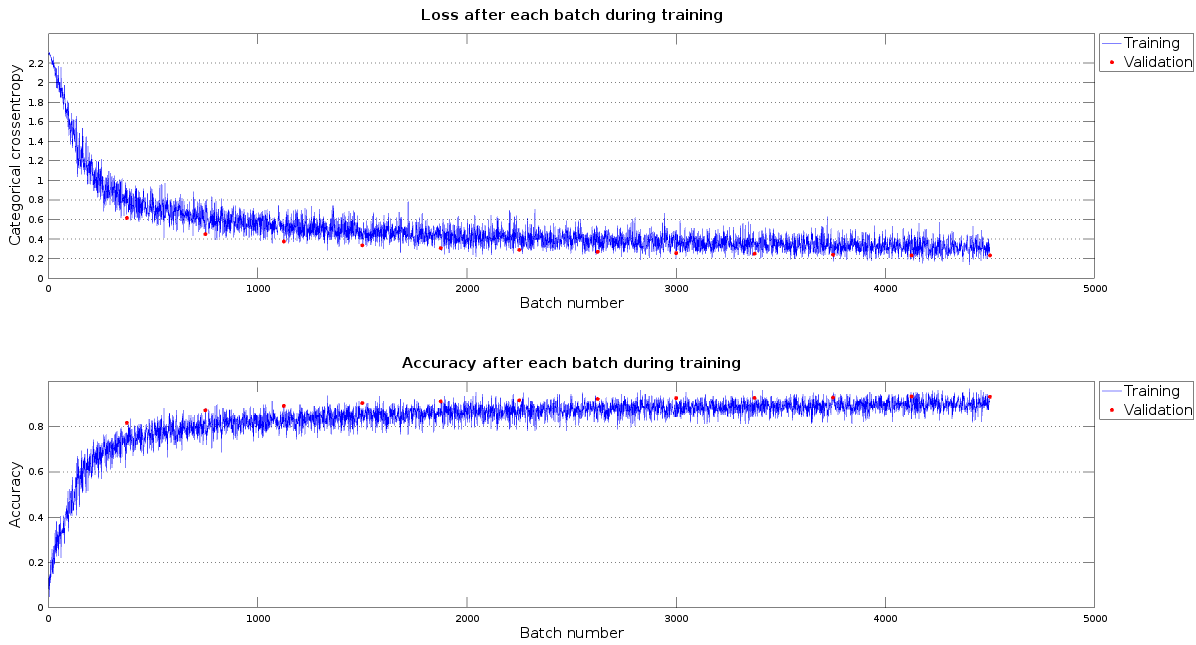
\includegraphics[width=1\linewidth]{figures/learning_curves.png}
		\caption{Learning curves.}
	\end{subfigure}
	\begin{subfigure}{0.5\textwidth}
		\centering
		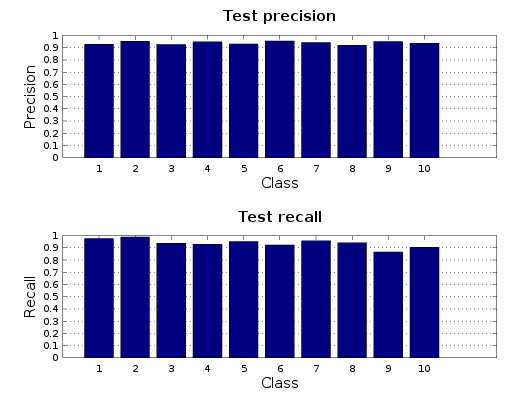
\includegraphics[width=0.9\linewidth]{figures/prec_rec.png}
		\caption{Precision and recall.}
	\end{subfigure}%
	\begin{subfigure}{0.5\textwidth}
		\centering
		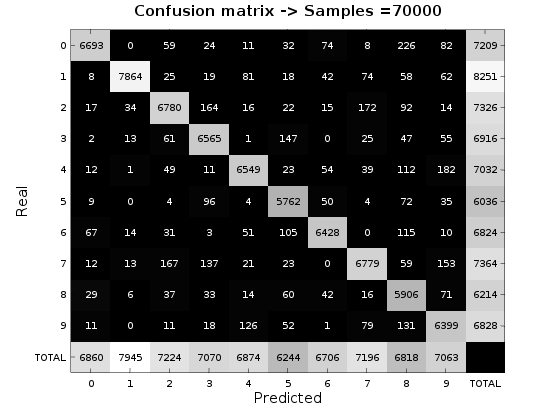
\includegraphics[width=0.9\linewidth]{figures/conf_mat.png}
		\caption{Confusion matrix.}
	\end{subfigure}
	\caption[Example of usage of \textit{benchmark.m}.]{}
	\label{fig:benchmark}
\end{figure}

\section{Visualizing the convolutional layer}
\glspl{cnn} are well-known by their ability of learning \textbf{image features}. The weights of a convolutional layer are arranged like \textbf{a set of filters}, each of which learns to identify a certain visual feature~\cite{cs231n}. As the filter is convolved with the input image, it generates an \textbf{activation map} that will tell us how that particular filter reacts to that image. In other words, the activation map will tell us whether a certain feature is present in the image or not.

In order to understand how the Keras model is learning to classify the digits, the script \textbf{\textit{layer\_visualization.py}}~\footnote{\url{https://git.io/vH94o}} has been written. This script displays the filters that are learned in every convolutional layer of the model and their resulting activation maps. The images that are going to be analyzed in the following sections correspond to the \textit{2conv$+$MaxPooling} model trained with the dataset 0-1 with early stopping (see Section~\ref{subsec:arch}) 

\subsection{Filters}
Accessing the weights of the layers in a Keras model is as easy as loading the model and calling the methods \textit{model.get\_layer("name")} and \textit{layer.get\_weights()}. When loading the weights of the \textbf{first convolutional layer}, a Numpy array of shape (1, 3, 3, 32) is obtained. This means that the weights are arranged in 32 filters of size 3x3. In this case, the input is a grayscale image, so the filters only have one channel (i.e. depth=1). Besides that, when examining their values, \textbf{negative and positive coefficients} are found.

In Figure~\ref{fig:filters}, these filters are plotted. Some of the filters look too noisy to tell which kind of feature they are looking for. However, a few of them can be interpreted as folllows:
\begin{itemize}
	\item \textbf{Horizontal edges}: filters 7, 9 and 23.
	\item \textbf{Vertical edges}: filters 8, 15 and 31.	
\end{itemize}

\begin{figure}
	\centering
	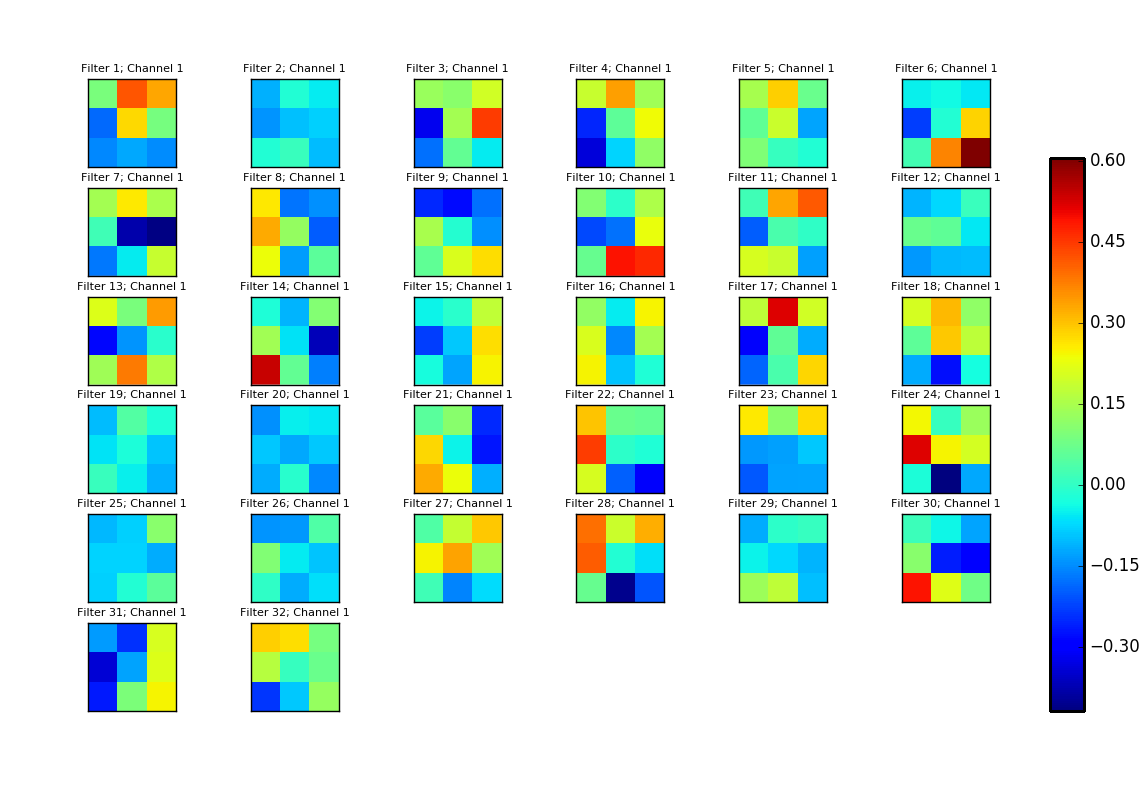
\includegraphics[width=0.85\linewidth, keepaspectratio]{figures/weights_conv2d_1.png}
	\caption{Filters of the first convolutional layer.}
	\label{fig:filters}
\end{figure}

The filters in the \textbf{second convolutional layer} have been analyzed as well. The shape of the weights in this layer is (32, 3, 3, 32), which means that there are 32 filters with size 3x3. This time, its depth is 32, since there is one channel per activation map generated by the previous layer. As we get \textbf{deeper in the \gls{cnn}} and the dimensionality grows, the filters look noisier and become harder to interpret, as it can be seen in Figure~\ref{fig:filters2}.
\begin{figure}
	\centering
	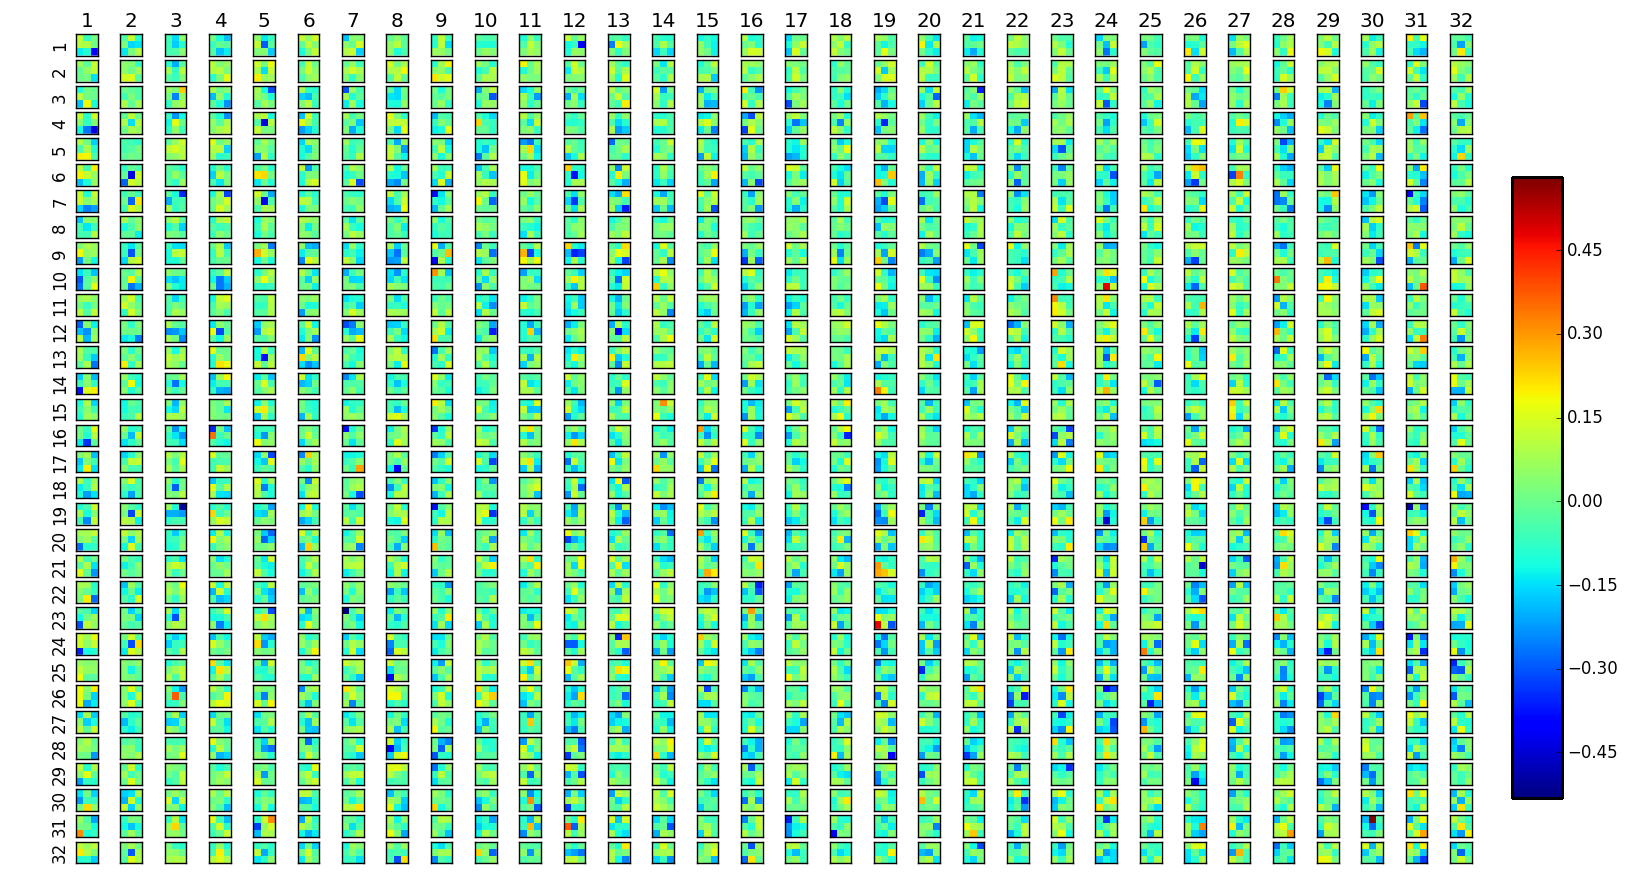
\includegraphics[width=1\linewidth, keepaspectratio]{figures/weights_conv2d_2.png}
	\caption[Filters of the second convolutional layer.]{Filters of the second convolutional layer. Each row contains the channels (1-32) that correspond to each filter (1-32).}
	\label{fig:filters2}
\end{figure}

\subsection{Activation maps}
The output of each convolutional layer is formed by as many \textbf{activation maps} as filters have the layer. In order to get the values of these activation maps, \textbf{truncated versions} of the original model have been generated, as it can be seen in Figure~\ref{fig:truncated}. If a prediction is made with these truncated models, they will output the activation maps that correspond to their last layer.
\begin{figure}
	\begin{subfigure}{0.5\textwidth}
		\centering
		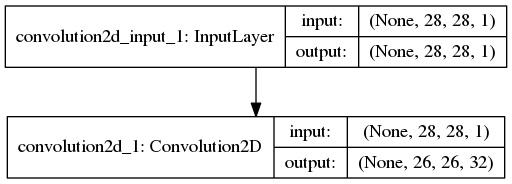
\includegraphics[width=0.9\linewidth]{figures/1stconvarch.png}
		\caption{}
	\end{subfigure}
	\begin{subfigure}{0.5\textwidth}
		\centering
		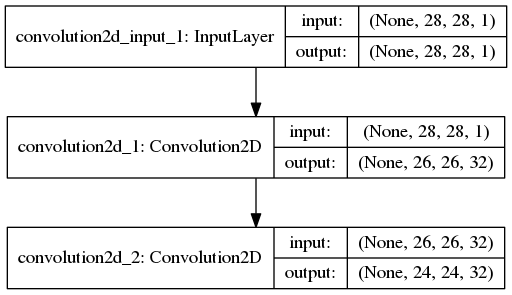
\includegraphics[width=0.9\linewidth]{figures/2ndconvarch.png}
		\caption{}
	\end{subfigure}
	\caption{Truncated versions of the model.}
	\label{fig:truncated}
\end{figure}

Figure~\ref{fig:activation_maps} shows the activation maps that the \textbf{first convolutional layer} of the model outputs. There are \textbf{horizontal and vertical edge images} that confirm the interpretation of the filters given in the previous section. Besides that, some activation maps (2, 12, 19, 25 and 26) look \textit{dead}. If we look back into Figure~\ref{fig:filters}, these activation maps correspond to filters with \textbf{almost flat coefficients}. This may be a signal of a high learning rate~\cite{cs231n}. In this case, the learning rate is not explicitly declared: the ADADELTA optimizer \ref{adadelta} use an adaptive one.
\begin{figure}
	\centering
	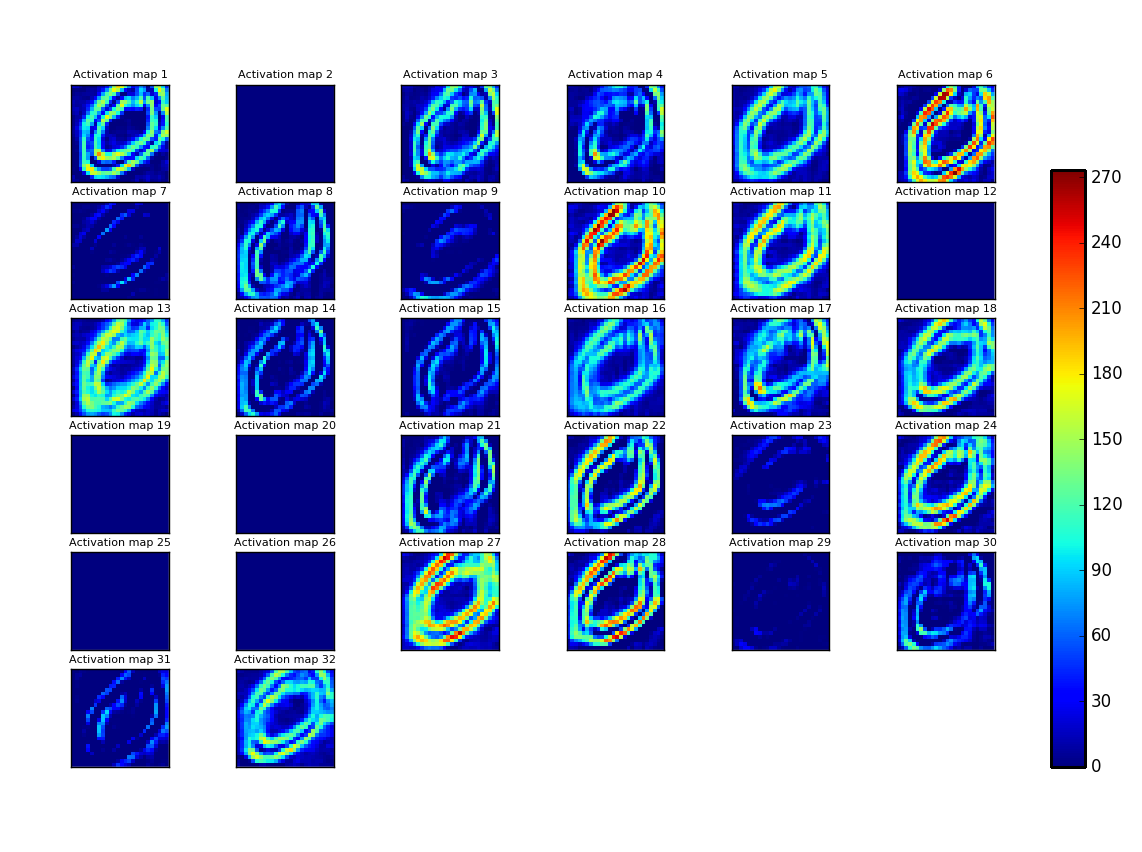
\includegraphics[width=0.85\linewidth, keepaspectratio]{figures/activation_maps_conv2d_1.png}
	\caption{Activation maps of the first convolutional layer.}
	\label{fig:activation_maps}
\end{figure}

The activation maps of the \textbf{second layer} are shown in Figure~\ref{fig:activation_maps2}. The images obtained look \textbf{more specialized} than the ones in the previous layer. It's easier to tell to what kind of feature (e.g. edges and corners) each activation map is responding to.
\begin{figure}
	\centering
	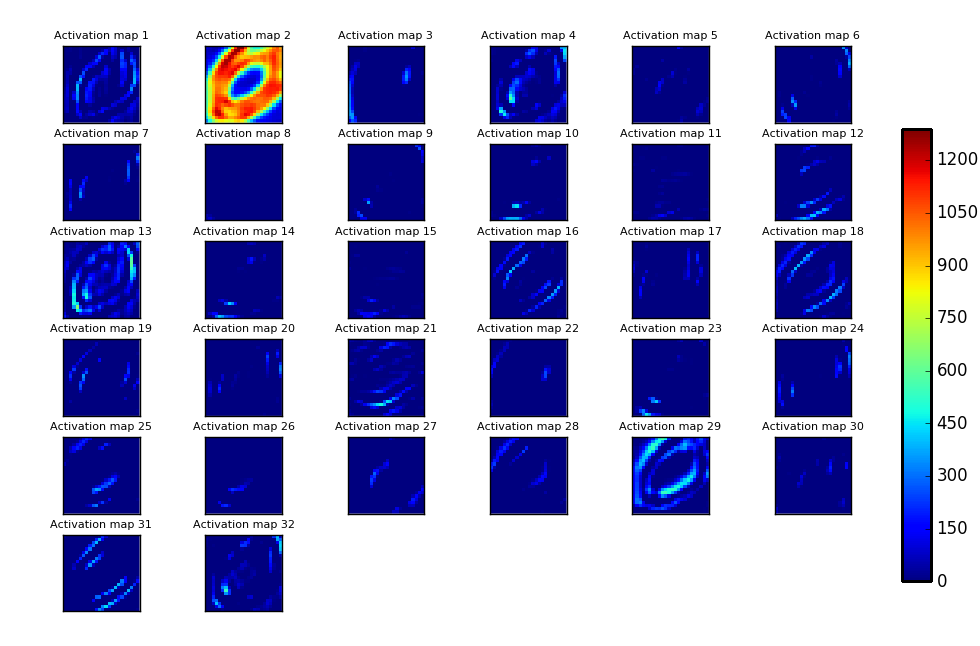
\includegraphics[width=0.85\linewidth, keepaspectratio]{figures/activation_maps_conv2d_2.png}
	\caption{Activation maps of the second convolutional layer.}
	\label{fig:activation_maps2}
\end{figure}

It's important to note that the values of the activation maps are \textbf{always positive}, even if the filters have negative coefficients. This is because the \gls{relu} activation function (see Equation~\ref{eq:relu}) turn all the negative values to zero.

\section{Evaluation}\label{sec:new_models}
The \gls{cnn} analyzed in Section~\ref{sec:classifier} is going to be taken as a starting point to build \textbf{new models}. These models will be trained with \textbf{different datasets} and \textbf{regularization methods} and, finally, \textbf{new architectures} will be implemented. During this process, the tools developed in Section~\ref{sec:bencharmk} will be employed to evaluate the results achieved by each model.

\subsection{Different datasets}
The original model has been trained with each of the \textbf{handmade datasets} described in Section~\ref{sec:datasets}. The number of epochs has been set to 12 and the evaluation has been carried out with the \textbf{1-6 test dataset}. The results that can be seen in Table~\ref{tbl:datasets} lead to the following conclusions:
\begin{itemize}
	\item As it might be expected, the results when training with the \textbf{Sobel dataset} are much worse than the ones obtained with the other datasets, because we're testing with noisy images a \gls{cnn} trained with noiseless samples.
	\item The \textbf{\textit{0-6} and \textit{1-6} models} are the ones that achieve better results, as they have been trained with \textbf{six times more samples} than \textit{0-1} and \textit{1-1}.
	\item When \textbf{comparing \textit{0-1} with \textit{1-1} and \textit{0-6} with \textit{1-6}}, it can be seen that the performance is almost the same, which means that the \textbf{gradient image without noise and transformations} is not adding much information to the model.
\end{itemize}

Taking all of this into account, it has been decided to keep working with the \textbf{\textit{0-1} model}, which achieves a performance that is comparable with the other models with the advantage of a much lower computational cost.

\begin{table}
	\centering
	\begin{tabular}{l*{4}{c}r}
		\textbf{Model} & \textbf{Loss} & \textbf{Accuracy} & \textbf{Epochs} \\
		\hline
		Sobel & 1.233 & 0.699 & 12 \\
		0-1 & 0.201 & 0.939 & 12 \\
		1-1 & 0.189 & 0.943 & 12 \\
		0-6 & 0.109 & 0.968 & 12 \\
		1-6 & 0.111 & 0.967 & 12 \\
	\end{tabular}
	\caption{Results of training with different datasets.}
	\label{tbl:datasets}
\end{table}

\subsection{Regularization methods}
"\textbf{Regularization} is any modification we make to a learning algorithm that is intended to reduce its \textbf{generalization error} but not it's \textbf{training error}"~\cite{Goodfellow-et-al-2016}. Reducing the generalization error is important because, even if a model achieves a great accuracy or loss with the training dataset, if it doesn't generalize well enough, the results during validation and test time won't be optimal. This is specially significant in our case, since the predictions of the digit classifier will be based on \textbf{images that differ a lot from the train dataset}. In this section, the effect of applying to the \textit{0-1} model two regularization techniques (\textbf{early stopping} and \textbf{dropout}) is going to be evaluated. 

\subsubsection{Early stopping}
The models in the previous section have been trained for 12 epochs. However, if we look at the \textbf{validation results} in Figure~\ref{fig:val_datasets}, the models were \textbf{not overfitting} yet, because the results didn't stop improving. This means that they were not being trained as much as possible. Setting an early stopping rule (see Section~\ref{subsec:callbacks}) allows training the \gls{cnn} right until it starts to overfit, making the most of it. The criteria that has been used depends on the loss during validation. The model is trained until the log-loss (see Section~\ref{eq:categorical_crossentropy}) has not improved after two validations in a row, i.e. a patience of 2. Besides that, in order to keep the best \textit{version} of the model, the log-loss is checked after each epoch and if it's the lower than the previous best log-loss achieved, the weights of the model are saved, overwritting the weights of the previous best \textit{version}. The difference between training the model with and without early stopping can be seen in Table~\ref{tbl:earlystopping}.
\begin{figure}
	\centering
	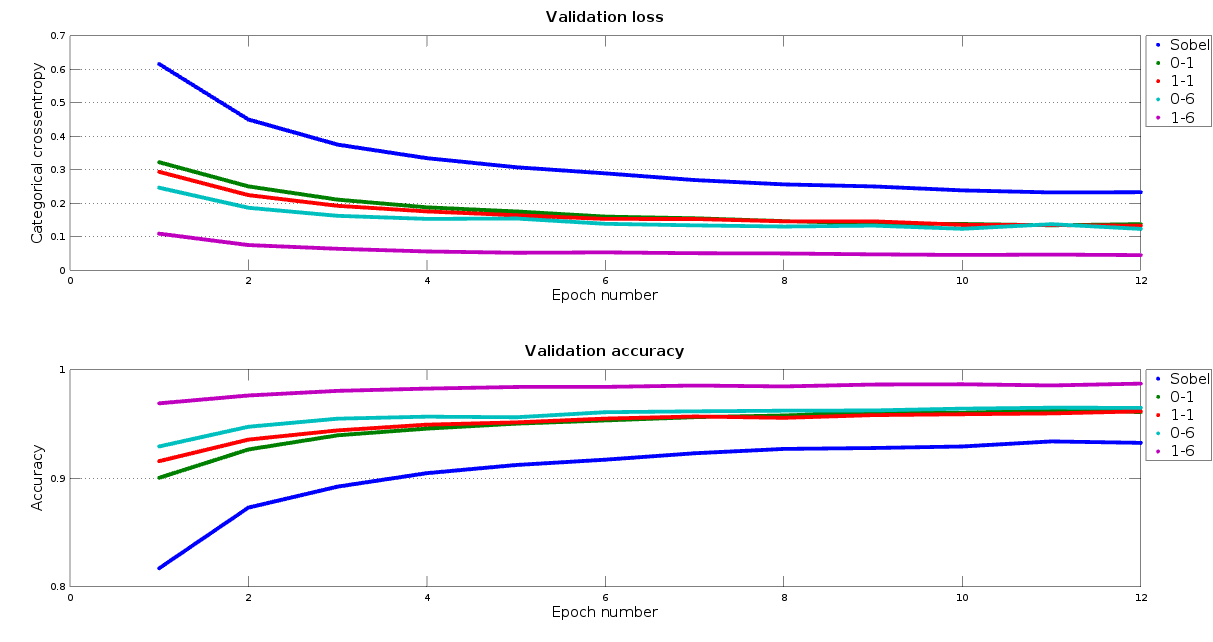
\includegraphics[width=1\linewidth, keepaspectratio]{figures/val_datasets.png}
	\caption{Validation results when training the model with different datasets.}
	\label{fig:val_datasets}
\end{figure}

\begin{table}
	\centering
	\begin{tabular}{l*{4}{c}r}
		\textbf{Model} & \textbf{Loss} & \textbf{Accuracy} & \textbf{Epochs} \\
		\hline
		0-1 & 0.201 & 0.939 & 12 \\
		0-1; Patience 2 & 0.155 & 0.954 & 30 \\
	\end{tabular}
	\caption{Results of training with and without early stopping.}
	\label{tbl:earlystopping}
\end{table}

Early stopping means an improvement of 1.6\% in accuracy and 4.6\% in log-loss. The model has been trained for 30 epochs and reached its best \textit{version} at the 27$^{th}$ epoch. Setting a longer patience has been considered, but it has been decided to apply it only to the best model obtained after Section~\ref{subsec:arch} to reduce the computational cost.

\subsubsection{Dropout}
The models that we're working with insert dropout (see Section~\ref{subsec:layers}) before every dense layer of the \gls{cnn} (0.25\% and 0.5\%, respectively). Dropout is usually applied just to fully connected or dense layers, because convolutional layers are less likely to overfit due to their architecture. In order to determine how dropout affects the performance of the model, the \textit{0-1; Patience 2} dataset has been trained with and without the mentioned dropout. The results can be seen in Table~\ref{tbl:dropout}. 
\begin{table}
	\centering
	\begin{tabular}{l*{4}{c}r}
		\textbf{Model} & \textbf{Loss} & \textbf{Accuracy} & \textbf{Epochs} \\
		\hline
		No dropout & 0.189 & 0.945 & 9 \\
		Dropout & 0.155 & 0.954 & 30 \\
	\end{tabular}
	\caption{Results of training with and without dropout.}
	\label{tbl:dropout}
\end{table}

Without dropout, the model has stopped training after 9 epochs. It has learned faster, but it has started overfitting earlier, resulting in worst results that the ones achieved by the model trained with dropout. This can be clearly seen in Figure~\ref{fig:comp_dropout}
\begin{figure}
	\centering
	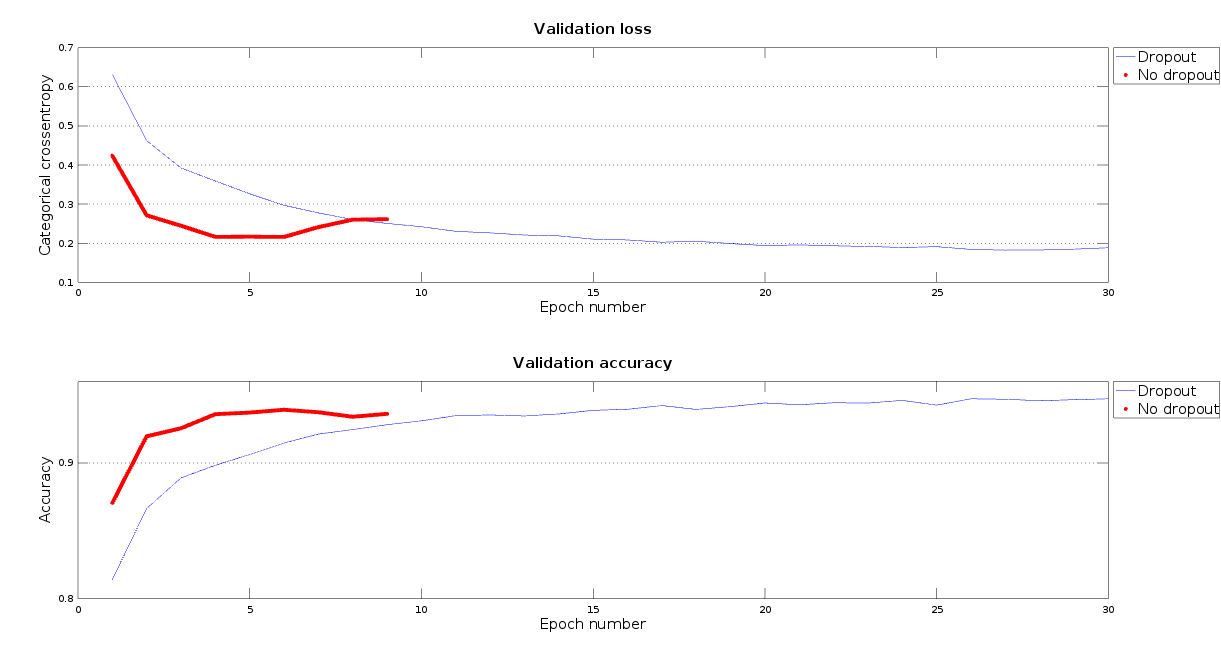
\includegraphics[width=1\linewidth, keepaspectratio]{figures/comp_dropout.png}
	\caption{Validation results with and without dropout.}
	\label{fig:comp_dropout}
\end{figure}

Additionally, in Figure~\ref{fig:lc_dropout}, the learning curves of the models can be seen. It's worth looking into these plots to realize that validation results are better than training results when the model is trained with dropout. This may look illogical, as the \gls{cnn} should always perform better with samples that it has already seen. However, it's important to remember that dropout only applies during training and, as it will \textit{switch off} a lot of weights in the \gls{cnn}, much of its prediction power will be lost. During validation, there are no \textit{switched off} weights, which allows the \gls{cnn} to make better predictions. Besides that, in the figure can be seen that the training results are much better (i.e. lower loss and higher accuracy) when the model is trained without dropout, while the validation results are better with dropout. This means that the model with dropout is generalizing better than the one without dropout. 
\begin{figure}
	\begin{subfigure}{1\textwidth}
		\centering
		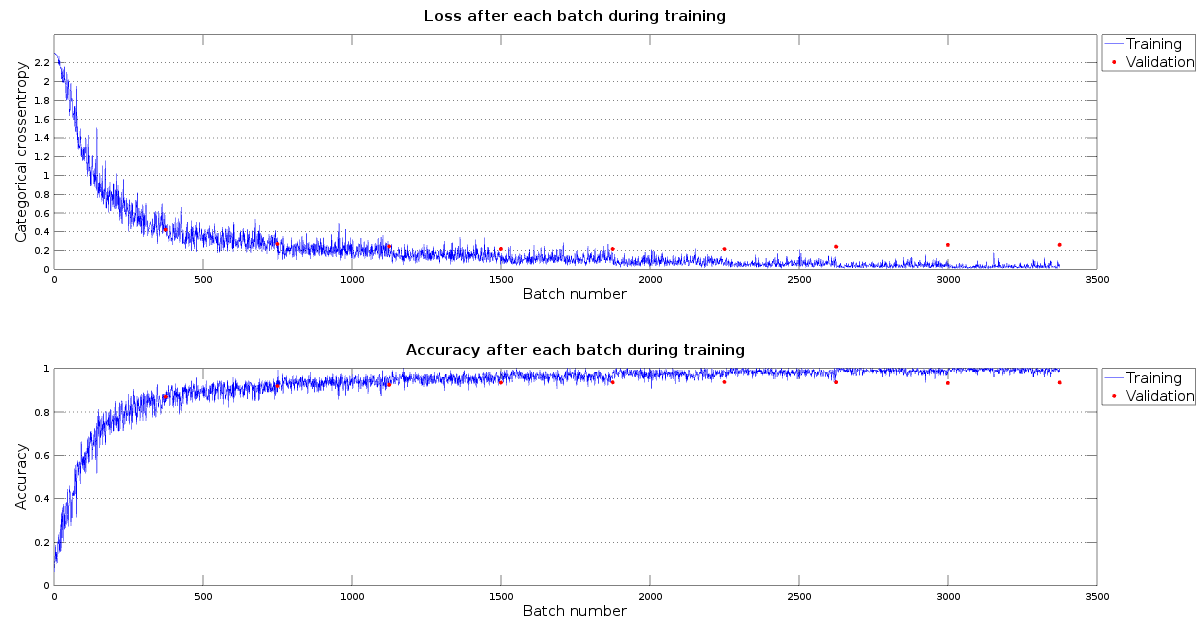
\includegraphics[width=1\linewidth]{figures/lc_nodropout.png}
		\caption{Learning curves without dropout.}
	\end{subfigure}
	\begin{subfigure}{1\textwidth}
		\centering
		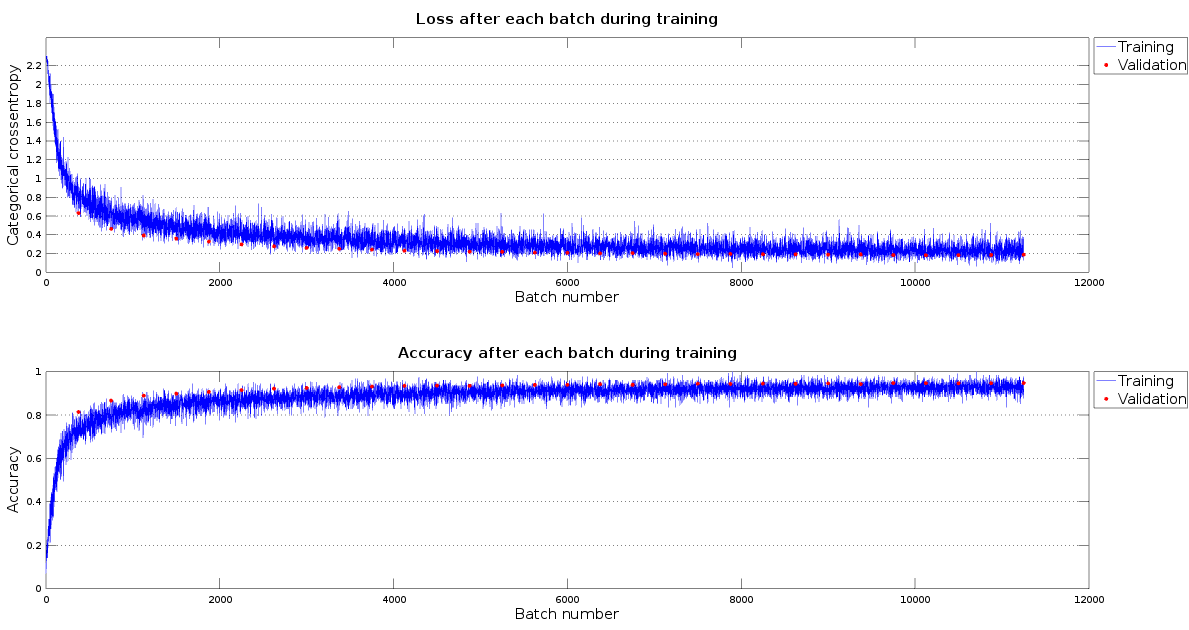
\includegraphics[width=1\linewidth]{figures/lc_dropout.png}
		\caption{Learning curves with dropout.}
	\end{subfigure}
	\caption[Learning curves with and without dropout.]{}
	\label{fig:lc_dropout}
\end{figure}

\subsection{Different architectures}\label{subsec:arch}
In order to check the influence of different architectures in the performance of the \gls{cnn}, new models with a different number of convolutional layers have been trained and tested. The stopping rule used in these trainings is the one defined in the previous section and dropout is also applied. The decision of adding pooling layers to the models (see Section~\ref{subsec:layers}) has been taken to reduce computational cost. In the first attempt at training a model with 6 convolutional layers, I triplicated the model with 2 convolutional layers and one MaxPooling layer. However, a MaxPooling layer was removed because the model ended up working with an empty image: 0x0 size.
\begin{table}
	\centering
	\begin{tabular}{l*{4}{c}r}
		\textbf{Model} & \textbf{Loss} & \textbf{Accuracy} & \textbf{Epochs} \\
		\hline
		1Conv+MaxPooling & 0.191 & 0.945 & 47 \\
		2Conv+MaxPooling & 0.155 & 0.954 & 30 \\
		3Conv+MaxPooling & 0.129 & 0.945 & 28 \\
		2Conv+MaxPooling+2Conv+MaxPooling & 0.092 & 0.970 & 27 \\
		4Conv+MaxPooling+2Conv+MaxPooling & 0.092 & 0.971 & 24 \\
	\end{tabular}
	\caption{Results of training models with different architectures.}
	\label{tbl:arch}
\end{table}

As it can be seen in Table~\ref{tbl:arch}, the best results have been obtained with the models that contain 4 and 6 convolutional layers. Besides that, taking a look into the validation curves (see Figure~\ref{fig:comp_arch}), it can be assumed that when we increase the number of layers, the neural network tends to lead to better results with less epochs.

\begin{figure}
	\centering
	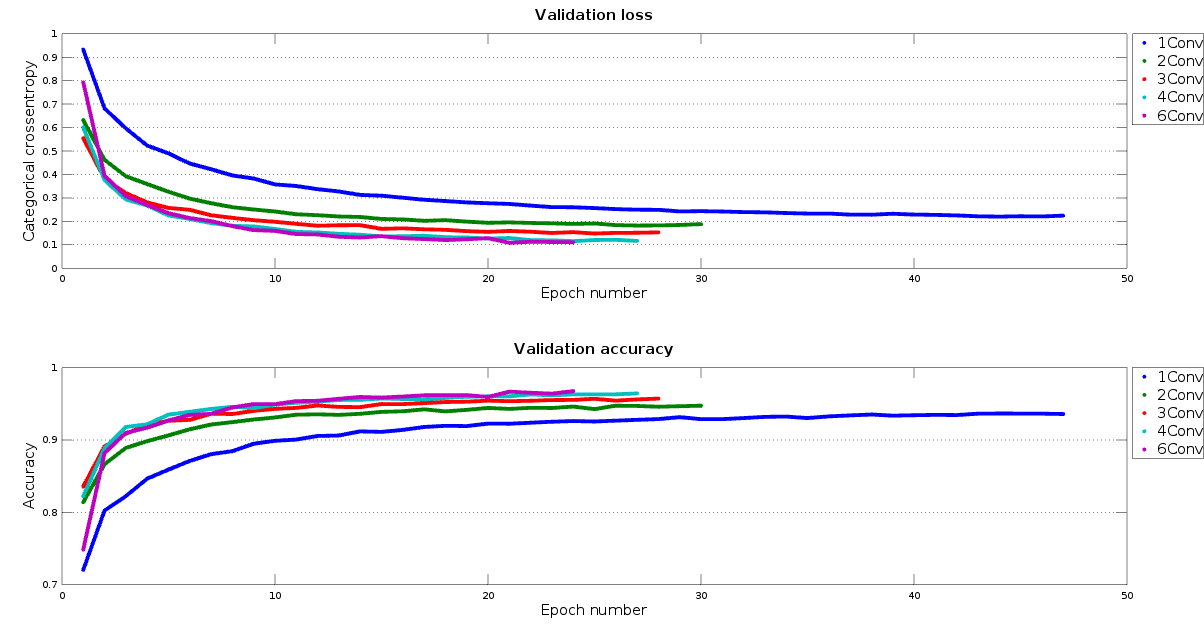
\includegraphics[width=1\linewidth, keepaspectratio]{figures/full_comparison.png}
	\caption{Validation results with different architectures.}
	\label{fig:comp_arch}
\end{figure}

The model with 6 layers has a slightly better accuracy but a slightly worse loss than the one with 4 layers. Considering that computational cost is higher when training the \textit{6Conv} model, \textit{4Conv} model seems to be the best bet. In order to make the most of it, it has been trained again but increasing the patience of the early stopping from 2 to 5. The results obtained with the new stopping rule can be seen in Table~\ref{tbl:arch_patience5}. These results imply that being more \textit{patient} during training can lead to a better performance, although in this case the improvement is not very significant.
\begin{table}
	\centering
	\begin{tabular}{l*{4}{c}r}
		\textbf{Model} & \textbf{Loss} & \textbf{Accuracy} & \textbf{Epochs} \\
		\hline
		4Conv; Patience 2 & 0.092 & 0.970 & 27 \\
		4Conv; Patience 5 & 0.082 & 0.973 & 37 \\
	\end{tabular}
	\caption{\textit{4Conv} model trained with different stopping rules.}
	\label{tbl:arch_patience5}
\end{table}